\documentclass{article}
\usepackage{amsmath, graphicx, amsfonts, caption, subfig, keyval, algorithm, algorithmic}
\newcommand{\R}{\mathbb{R}}

\begin{document}
\title{Optimizing Distribution Center Placement}
\author{Jonathan Friedman \& Taylor Killiam}
\maketitle

%TODO before submission: make everything pretty and readable

\section{Introduction} \label{introduction}
Serving the maximum number of people at minimum expense is an important and general problem in industry. A company must balance placing their distribution centers near as many people as possible with the cost associated with opening and maintaining a large number of centers. In this paper, we examine the problem of placing distribution centers so that a specified cost function, such as average distance from a center, is below a given threshold. 

This problem is easy to solve for one center. In section \ref{onecenter}, we give a solution for one point using compass search. However, compass search is not viable for a large number of points because the number of required directions to search grows at least quadratically(???). Instead, we use a clustering-based algorithm as described in \ref{multicenters}.
%TODO: Add more detailed explanation of what we're doing.

In section \ref{experiments}, we use our algorithm to optimize placement of points of service in Massachusetts based on population data from the U.S. 2010 Census \cite{census}.

\section{One Distribution Center} \label{onecenter}
Compass search is a simple method of minimizing a function $f \in \R^n$. The algorithm is described in Algorithm \ref{alg:compass} (see \cite{survey} for details).

\begin{algorithm}
  \caption{Compass Sort}
  \label{alg:compass}
\begin{algorithmic}
  \STATE  Choose $\lambda_1,...,\lambda_m$ to be a positive spanning set of $\R^n$. Choose a starting guess $p_0$, a step size $s_0$, a scaling constant $\alpha<1$, and a tolerance $t$.
  \WHILE{$s_k > t$}
  \IF{$f(p_k + s_k\lambda_i) < f(p_k)$ for some $\lambda_i$}
  \STATE $p_{k+1} = p_k + s_k\lambda_i$
  \STATE $s_{k+1} = s_k$
  \ELSE
  \STATE $p_{k+1} = p_{k}$
  \STATE $s_{k+1} = \alpha s_k$
  \ENDIF
  \ENDWHILE
  \RETURN $p_{k+1}$
\end{algorithmic}
\end{algorithm}

In general, we minimize $$\sum_i f(\alpha_i) d(p, q_i)$$ where $p$ is the location of the point of service, $\alpha_i$ and $q_i$ are the population at and location of point $i$, $f$ is a function that weights the population, $d$ is a distance function, and the sum is over all points for which we have population data (in practice, because there are around 160,000 census blocks in Massachusetts, we subsample the population data to achieve better performance). Figure \ref{fig:popscale} shows point-of-service placement for various $f$, with $d(p-q_i) = ||p - q_i||_2$.

%TODO: make this figures actually readable by making point of service larger and removing key
\begin{figure}%
  \centering
  \subfloat[$f(\alpha_i)=\alpha_i$]{{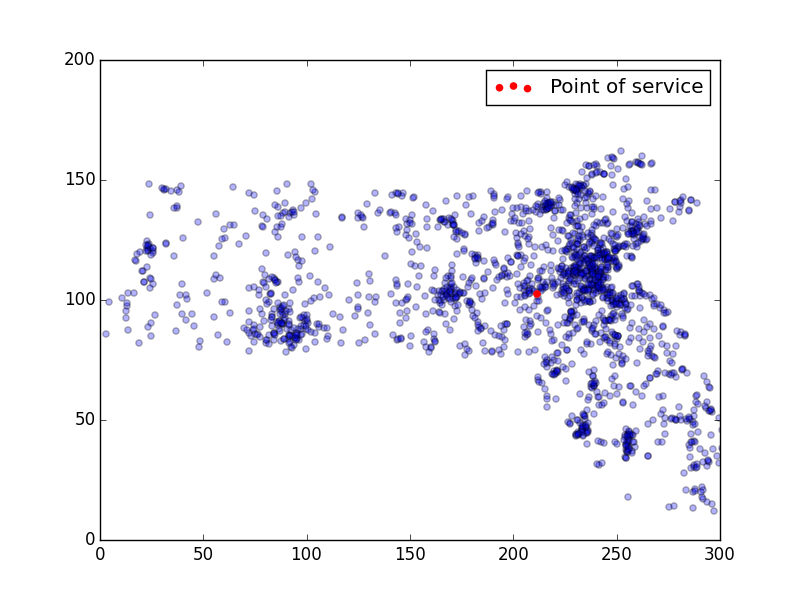
\includegraphics[width=5cm]{popscale.png} }}%
  \qquad
  \subfloat[$f(\alpha_i)=\sqrt{\alpha_i}$]{{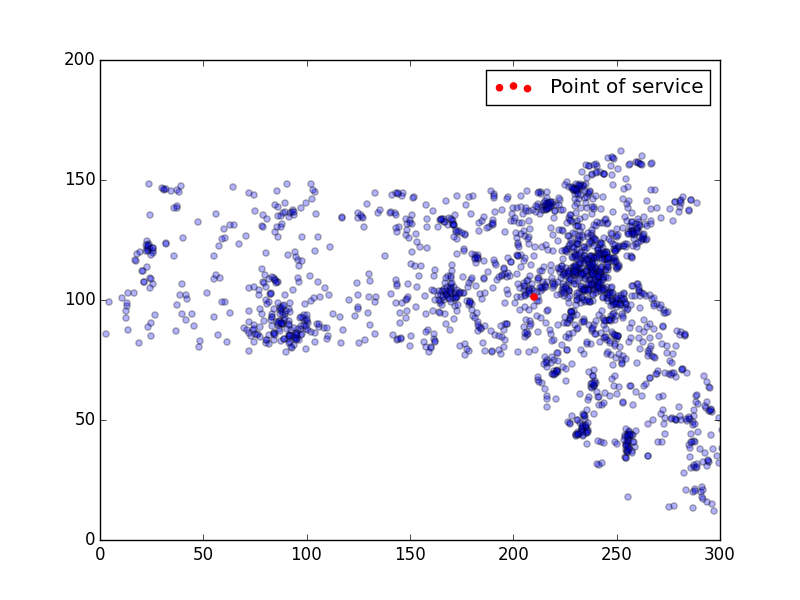
\includegraphics[width=5cm]{sqrtpopscale.png} }}%\\
  \qquad
  \subfloat[$f(\alpha_i)=\alpha_i^2$]{{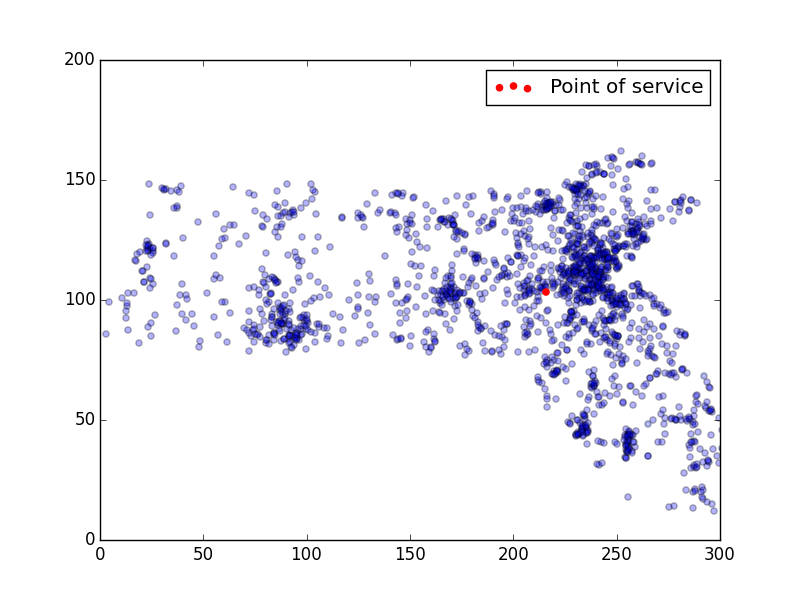
\includegraphics[width=5cm]{squarepopscale.png} }}%
  \qquad
  \subfloat[$f(\alpha_i)=\alpha_i^4$]{{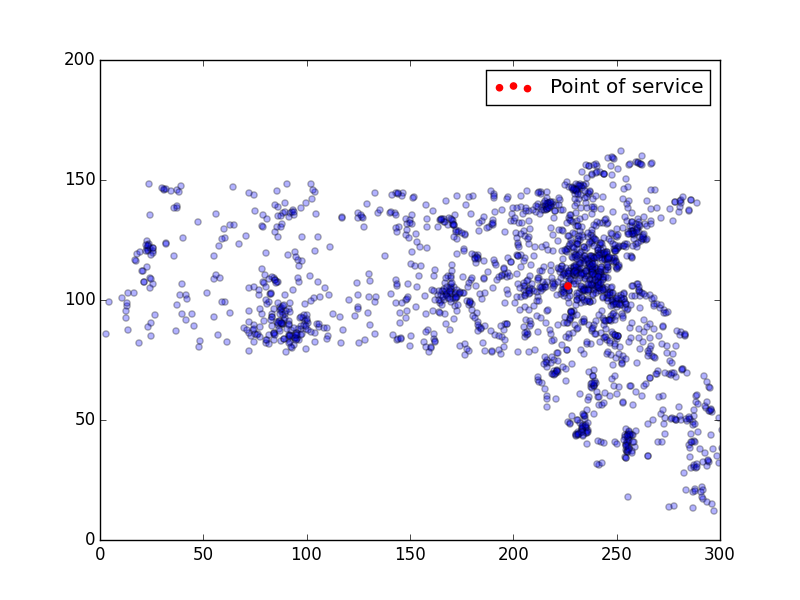
\includegraphics[width=5cm]{fourthpopscale.png} }}%
  \caption{Distribution center placement under \\ various population scaling functions}
  \label{fig:popscale}
\end{figure}

This method works well for one point of service, but the number of directions to search grows at least quadratically with the number of points.  Consider the case of two points $p_1, p_2 \in \R^2$. Our function to minimize is now $$\sqrt{\sum_i f(\alpha_i)\min(g(p_1, q_i), g(p_2, q_i))}$$ which corresponds to minimizing each person's distance from the nearest point of service. A positive spanning set for $\R^n$ must contain at least $n+1$ vectors \cite{charles}, so we must consider at least 3 possible directions at each step for $p_1$ and $p_2$. For simplicity, consider the non-minimal positive spanning set of the four cardinal directions. IT IS BAD AND NOT GOOD SCALING.

% TODO: figure out how fast it actually scales
%The algorithm is then to find a direction for $p_1$ that produces a decrease, then find a direction for $p_2$ that produces a decrease. Even if the first possible direction evaluated for $p_1$, then the first possible direction for $p_2$, yield decreases,

\section{Multiple Distribution Centers} \label{multicenters}
% TODO: Describe clustering algorithm
\section{Experiments} \label{experiments}
%TODO: Describe we collected, parsed, subsampled, etc. census data.

\begin{thebibliography}{9}
  \bibitem{census}
  U.S. Census Bureau. \textit{TIGER/Line� with Selected Demographic and Economic Data: Population \& Housing Unit Counts}, 2010 Census. Nov. 9, 2015. https://www.census.gov/geo/maps-data/data/tiger-data.html.
  \bibitem{survey}
  Cite survey on optimization here
  \bibitem{charles}
  Cite "Theory of Positive Linear Dependence" here
\end{thebibliography}
\end{document}